%!TEX root = ../index.tex

\newpage
\section{Mobile Applikation} % (fold)
\label{sec:Mobile Applikation}

\subsection{Vorbereitung} % (fold)
\label{sub:Vorbereitung}
\subsubsection{Marktanalyse} % (fold)
\label{ssub:Marktanalyse}
Zur Zeit ist in der Schweiz das iPhone das meist verkaufte Smartphone. Dies und der App Store von Apple sind Gründe, weswegen viele Unternehmen ihre Mobileapplikationen erst für das iPhone entwickeln. Zur Zeit wächst jedoch der Android Markt sehr schnell und wird das iPhone wahrscheinlich vom ersten Platz verdrängen. Das Entwickeln einer App für Android ist jedoch in einigen Punkten komplexer als es für das iPhone ist, da die Diversität der Geräte massiv höher ist und kaum ein Gerät auf einen Relevanten Marktanteil kommt. Daher ist es zur Zeit sinnvoll eine iPhone Anwendung für mehrere Geräteklassen zu entwickeln.
% subsubsection Marktanalyse (end)

\subsubsection{Plattformevaluation} % (fold)
\label{ssub:Plattformevaluation}
Da die Verfasser dieser Arbeit iOS und Android Geräte verwenden, wurde auf ein Crossplatform Framework gesetzt. Zum Zeitpunkt dieser Evaluation gab es zwei mögliche Wege, plattformunabhängige Applikationen zu erstellen.
\begin{itemize}
    \item Adobe Flex
    \item Phonegap
\end{itemize}
Da Phonegap bessere Unterstützung für exotische Plattformen hatte und es mit JavaScript auf einer Programmiersprache beruht welche auch im World Wide Web eingesetzt wird und Adobe Flex mit ActionScript3 auf eine Sprache setzt welche ausser in Adobe Produkten nicht eingesetzt wird, fiel die Entscheidung auf Phonegap
% subsubsection Plattformevaluation (end)
% subsection Vorbereitung (end)

\subsection{Geolocation Navtive Feature} % (fold)
\label{sub:geolocation_native_feature}
Von Geolocation Native Funktion werden zwei PhoneGap Methoden verwendet. Initial wird getCurrentPosition verwendet um die aktuelle Position festzustellen. Danach werden mit watchPostion Veränderungen festgestellt und abgespeichert. Die Ankunft von neuen Geolocation Daten löst immer direkt eine Berechnung der Abstände und Richtungen zu den Zielen aus. Der Wert den die Methoden zurückliefern ist die Gradangabe unterschiedlich von Nord. Daher ist Ost 90, Süd 180 und West 270.
% subsection geolocation_native_feature (end)

\subsection{Kompass Native Feature} % (fold)
\label{sub:kompass_native_feature}
Von der Kompass Native Funktion werden zwei PhoneGap Methoden verwendet. Mit getCurrentHeading wird die initiale Richtung festgestellt. Weiter wird mit watchHeading die Ausrichtung aktualisiert. Die Aktualisierung funktioniert in zeitlich bestimmten Abständen. Die Messungen sollten unter 500 Millisekunden sein um eine flüssige Applikation zu haben. Es ist jedoch darauf zu achten, das die Verarbeitungszeit nicht unterschritten wird, damit man nicht in Probleme mit zu vielen Verarbeitungen hinein läuft. Ein Update der Kompass-Daten löst immer eine Kalkulation der Signal-Stärke aus, welche im Zusammenhang mit der Richtung des Ziels (siehe Kapitel~\ref{sub:geolocation_native_feature}) und eingehenden Kompass-Richtung steht.
% subsection kompass_native_feature (end)

\subsection{Kalkulation} % (fold)
\label{sub:kalkulation}
\subsubsection{Richtung} % (fold)
\label{ssub:richtung}
Die Richtung wird mittels dem Öffnungswinkel zwischen den zwei Punkten berechnet und in Abhängigkeit zu Nord gebracht. So erhält man eine Richtung wie es die Kompass Native Funktion zurück liefert. Diese können dann direkt verglichen werden um die Korrektheit der Richtung und somit die Signalstärke ~\ref{ssub:signalstärke}
 festzustellen. 
% subsubsection richtung (end)
\subsubsection{Signalstärke} % (fold)
\label{ssub:signalstärke}
Die Signalstärke wird angezeigt, wenn die eigene Richtung näher wie 100 Grad an der Richtung des Ziels ist. In einer ersten Implementation wurde die Stärke linear berechnet. Daher: Wenn die Richtung um 99 Grad daneben war wurde 1\% Signalstärke angezeigt, bei 50 Grad waren es 50\% Signalstärke. Ein einem zweiten Schritt wurde die Signalstärke dann exponentiell berechnet. Daher: Bei kleiner Richtungsänderung in der nähe der perfekten Ausrichtung verändert sich die Signalstärke sehr stark, bei grösseren Richtungsänderungen im Bereich von 100 Grad Abweichung des Ziels verändert sich die Signalstärke nur schwach. Dieses Verhalten ist auch bei der Richtfunk-Fuchsjagd der Fall. Die Grösse mit den 100 Grad Abweichung kann mit einer guten Richtfunk Anlage ebenfalls bewerkstelligt werden. Schlechtere Anlagen haben einen grösseren Radius wo das Signal angezeigt wird und somit wird in allen Richtungen ein stärkeres oder schwächeres Signal festgestellt.
% subsubsection signalstärke (end)
\subsubsection{Distantz} % (fold)
\label{ssub:distantz}
Die Distanz wird mit einer Hypotenuse zwischen den beiden Punkten (Eigene Position und Ziel) mit den Deltas der Längen- und Höhenbreite berechnet. 
% subsubsection distantz (end)
% subsection kalkulation (end)

\subsection{Backend Kommunikation} % (fold)
\label{sub:backend_kommunikation}
Die Backend Kommunikation wurde längere Zeit mit statischen Zielen simuliert. Später sind dann die Daten zu den Zielen mit JSONP Requests vom Backend heruntergeladen worden. JSONP musste verwendet werden um das Problem von Cross Site Referenzen aus Java Script zu lösen, welches aus Security Gründen mit einfachem AJAX nicht machbar ist. Zurückgeliefert wird ein Java Script Array aus dem JSON Object.
% subsection backend_kommunikation (end)

\subsection{Stärkenanzeige} % (fold)
\label{sub:stärkenanzeige}
Für die Anzeige der Signalstärke für x Ziele wurde dynamisches HTML verwendet, was grundsätzlich keine schöne Lösung ist. Dabei werden mittels Java Script HTML Tags nach dem Laden für jedes gefundene Ziel ein HTML-Div in einen schon vorhandenen div eingebunden. Dabei erhält jeder der Divs eine individuelle dem Ziel angepasste ID damit die Signalstärke bei Änderungen angepasst werden können. Die Signalstärke wird von der Kalkulation in Prozent geliefert. Diese Prozentzahl kann dann direkt im HTML Signalstärke Tag width eingegeben werden, das die prozentuale Grösse vom darum liegenden Tag annimmt.
% subsection stärkenanzeige (end)

\subsection{Datenmanagement} % (fold)
\label{sub:datenmanagement}
Um die Daten der Ziele zu managen, wurde Objekt Orientiertes Java Script verwendet. Ein Ziel besitzt einen Namen, eine fixe Position, welche vom Backend geliefert wird, eine veränderliche Richtung und Entfernung. Zusätzlich besitzt das Objekt zwei Methoden. Die erste wird aufgerufen, wenn sich die eigene Position verändert. Sie berechnet die Distanz und Richtung und speichert diese dann direkt im Ziel-Objekt ab. Die zweite Methode wird aufgerufen, wenn sich die eigenen Richtung verändert, sie berechnet und liefert die neue Signalstärke direkt an den Aufrufer zurück. 
% subsection datenmanagement (end)

\subsection{Design} % (fold)
\label{sub:design}
Die dieser Arbeit vorliegende Applikation (siehe Screenshots) ist nicht mit Design ausgestattet. Zu oberst werden die eigene Längen- und Höhenbreite angezeigt. Darunter die eigene Richtung in Abweichung von Nord. 
Im unteren Teil der Applikation befindet sich eine Liste der Ziele, welche grün eingefärbt die Signalstärke für jedes Ziel anzeigt. Das Design soll in naher Zukunft angepasst werden, damit die Applikation ansprechender wird.
% subsection design (end)

\begin{figure}[H]
	\centering			      
        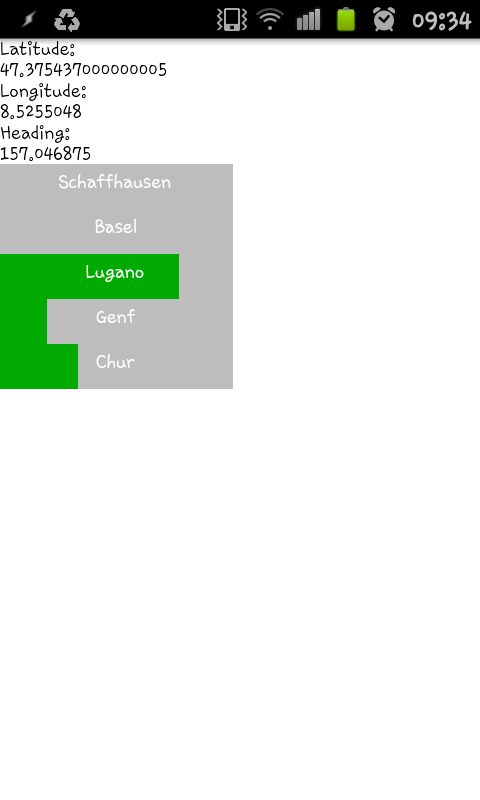
\includegraphics[scale=0.50, trim=0mm 15cm 0mm 0mm, clip]{images/screenshot-1.png}\\
		\caption{Screenshot}
	\label{fig:screenshot-1}
\end{figure}

\subsection{Mini-Kompass} % (fold)
\label{sub:mini_kompass}
Wie im Kapitel Design~\ref{sub:design} beschrieben, ist das Design und Frontend noch nicht ausgereift. Zusätzlich zu den Signalstärken zu den einzelnen Zielen, soll ebenfalls ein kleiner Kompass auf dem Bildschirm angezeigt werden. Dieser ist in der jetzigen Lösung nur als Grad Zahl in Abweichung von Nord angegeben. Somit braucht es für das spielen der Fuchsjagd lediglich noch eine Karte, die in Papierform den Vorteil der Übersicht und der Beschreibarkeit hat.
% subsection mini_kompass (end)

\begin{figure}[H]
	\centering			      
        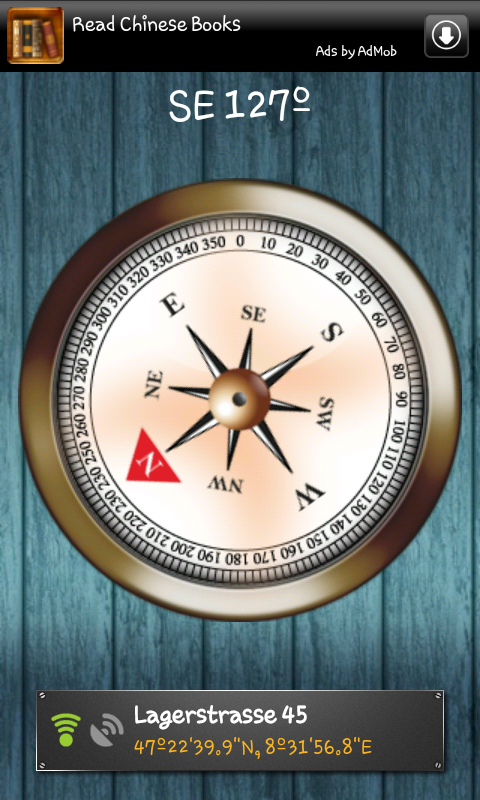
\includegraphics[scale=0.35, trim=5mm 6cm 5mm 6cm, clip]{images/kompass.png}\\
		\caption{Kompass}
	\label{fig:kompass}
\end{figure}
% section mobile applikation (end)
